\documentclass[main.tex]{subfiles}
\begin{document}

\section{Verbs}

The experiments described in this section explore the suitability of using verbal features for language classification. The English verb shows limited grammatical inflection, in contrast to the Spanish verb, which is heavily inflected for tense, mood, number, and person. English, nevertheless, does have a great deal of complexity in its verbal system, employing a wide range of auxiliary verbs and particles to indicate the various possible tense, aspect, and mood combinations, as well as other subtleties of meaning. It is not possible to provide a detailed description of the English verbal system here, but an attempt will be made to touch on the most salient aspects. As they occur rarely in written texts, particularly in the corpora used in this study, question and imperative forms are not discussed here.

\subsection{Grammar}

Not counting the verb \textit{to be}, English verbs have three finite inflected forms, as demonstrated here by the forms of the verb \textit{to walk}: a past tense form (\textit{walked}), a present third person singular form (\textit{walks}), and a form for all other present person/number combinations (\textit{walk}). This last form is also the base form of the verb, appearing in the infinitive after the particle \textit{to} (\textit{to walk}), and along with various auxiliary words to form the future (\textit{will walk}) and numerous other verbal constructions (\textit{should walk, am able to walk, have to walk}, etc.) In addition to the three finite forms, there is also a present participle (\textit{walking}) and a past participle (\textit{walked}), which is often identical to the past form.

The verb \textit{to be} has five finite forms, with three in the present: the first person singular \textit{am}, the third person singular \textit{is}, and \textit{are} for the other person/number combinations; and two in the past: \textit{was} for both first and third person singular, and \textit{were} for other cases. This latter form is also used in all persons and numbers for what is variously called the conditional or past subjunctive mood: (e.g. \textit{if I were rich\ldots}). In addition, there is the base form \textit{be}, the present participle \textit{being}, and the past participle \textit{been}.

In addition to these basic inflected forms, the English verbal system relies on a broad array of auxiliary words. One such class of words are the modal auxiliaries or, simply, the modals. The nine English modals are shown in Table~\ref{table:modal-verbs}. These modals express concepts as basic as the future and the subjunctive, and others more subtle, such as intention, obligation, ability, and so forth. It is important to note that these modals, whether they reflect a change of tense or not, do not inflect to agree with the subject. 

\begin{table}[htbp]
\small
\centering
\caption{English Verbal Forms Employing Modals}
\begin{tabular}{ r r r }
\toprule
\textit{will} walk & \textit{can} walk & \textit{should} walk \\
\textit{may} walk & \textit{could} walk & \textit{must} walk \\
\textit{might} walk & \textit{shall} walk & \textit{would} walk\\
\bottomrule
\end{tabular}
\label{table:modal-verbs}
\end{table}

Very similar to the modals are the phrasal modals. The thirteen phrasal modals considered in this experiment are those listed by \citet[Ch. 3]{quirk:1985}, and are shown in Table~\ref{table:quasimodal-verbs}. Of these, \textit{dare to}, \textit{need to}, \textit{have got to}, \textit{have to}, and all those beginning with the verb \textit{be}, can be inflected to show tense, person, and number, and can generally be used in conjunction with modals. The remaining phrasal modals do not inflect to agree with the subject, and are restricted to the present tense, with the exception of \textit{used to}, which is restricted to the past tense. It is worth noting that \citet{quirk:1985} do not group all of these into one category, but into three separate categories of modal-like auxiliaries: \textit{marginal modals}, \textit{modal idioms}, and \textit{semi-auxiliaries}. Because a more complicated analysis of these constructions would add little to this study, the term phrasal modal is here applied to any multiword modal-like construction.

\begin{table}[htbp]
\small
\centering
\caption{English Verbal Forms Employing Phrasal Modals}
\begin{tabular}{ r r r }
\toprule
\textit{dare to} walk & \textit{used to} walk & \textbf{be} \textit{about to} walk \\
\textit{need to} walk & \textit{had better} walk & \textbf{be} \textit{able to} walk \\
\textit{ought to} walk & \textit{have got to} walk & \textbf{be} \textit{bound to} walk \\
\textit{have to} walk & \textbf{be} \textit{supposed to} walk & \textbf{be} \textit{willing to} walk\\
&&\textbf{be} \textit{obliged to} walk\\
\bottomrule
\end{tabular}
\label{table:quasimodal-verbs}
\end{table}

The words \textit{have}, \textit{be}, \textit{get}, and \textit{do}, which are full verbs in their own right, play an important role in English as auxiliary verbs. When used as such, they become the inflected element of the verb, being used in conjunction with a nonfinite form of the main verb. A form of the verb \textit{have} followed by a past participle indicates the perfective aspect (e.g., \textit{he has walked/had walked/will have walked/}etc.) \textit{Be}, in any of its forms, plays two roles as an auxiliary. Followed by a present participle it forms the progressive aspect (e.g., \textit{he is walking/was walking/will be walking/}etc.) Followed by a past participle, it forms the passive mood (e.g., \textit{he was pursued.}) A passive can also be formed using \textit{get} plus a past participle (e.g. \textit{he got hurt}) A finite form of \textit{do} is used to add emphasis to a sentence and to form questions, negatives, and affirmative responses to questions, but only when no modal is present (e.g., \textit{you do not drink wine} but \textit{you will not drink wine}).

\subsection{Parsing of Verbs}

The Stanford Parser marks verbs, but does not explicitly mark all of the verbal attributes discussed above. The parse trees it generates indicate the structure of verb phrases (VPs), and distinguishes the various inflected forms of a verb. In general, it correctly distinguishes the finite and nonfinite uses of the base form of a verb. An example can be seen in Figure~\ref{fig:verb-parse}, which shows the parse of the sentence \textit{I do not want to go.} Here the three verbs \textit{do}, \textit{want}, and \textit{go} are tagged with the labels ``VBP,'' ``VB,'' and ``VB,'' respectively. ``VBP'' indicates a present form other than 3rd- person singular (which is indicated by ``VBZ''). ``VB'' marks a base form in a nonfinite usage. The parser also marks past-tense forms, \textit{ing}-forms, and \textit{ed}-forms, using ``VBD,'' ``VBG,'' and ``VBN,'' respectively. 

\begin{figure}[htbp]
\centering
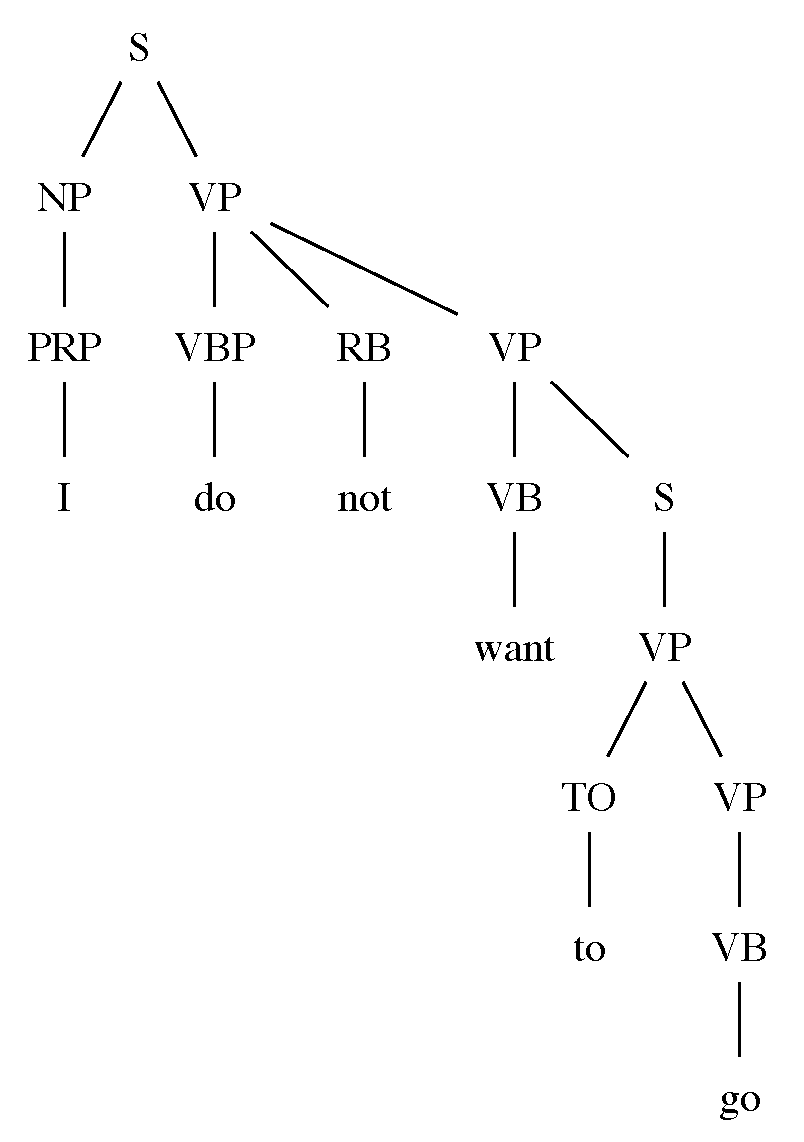
\includegraphics[scale=0.6]{verb-parse.pdf}
\caption{Typical Parse Tree Showing Verb Types.}
\label{fig:verb-parse}
\end{figure}

Any verbal information beyond that provided by these six tags must be determined from the shape and content of the VP subtrees in which the verbs are found. The parser directly marks modals, using the ``MD'' tag, as shown in Figure~\ref{fig:modal-parse}.
\begin{figure}[htbp]
\centering
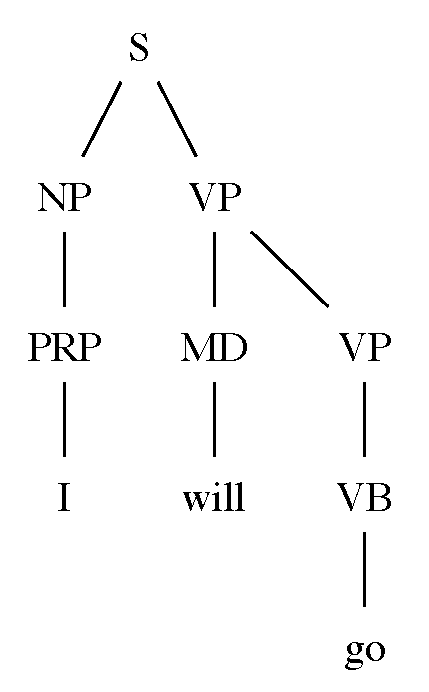
\includegraphics[scale=0.6]{modal-parse.pdf}
\caption{Parse Tree Showing Modal \textit{will}}
\label{fig:modal-parse}
\end{figure}
However, it does not mark phrasal modals in a consistent manner. Figures~\ref{fig:quasimodal-able} and \ref{fig:quasimodal-going} show how two phrasal modals are parsed differently. In Figure~\ref{fig:quasimodal-able}, \textit{he is able to go} is parsed with \textit{is} as the main verb, and with \textit{able to go} being an adjectival phrase. In Figure~\ref{fig:quasimodal-going}, the sentence \textit{he is going to go} is also parsed as a copular sentence, but with the predicate nominative being treated as a nonfinite clause. Indeed, the parser treats all phrasal modals of the form \textit{be}~+~particle~+~\textit{to} as \textit{be} verbs followed by an adjectival or participial construction. Perhaps this is not surprising as the distinction between these constructions and phrasal modals is somewhat blurry in English grammar. \citet[footnote, p. 144]{quirk:1985} indicate that the main criterion for distinguishing these is whether what follows \textit{be} is able to stand alone at the beginning of a sentence. Consider, for instance:
\eenumsentence{
\singlespacing
\item \textit{Compelled to take stern measures, the administration lost popularity.} \label{ex:compelled}
\item \textit{?Bound to take stern measures, the administration lost popularity.} \label{ex:bound}
\item \textit{Unable/Unwilling to resist, Matilda agreed to betray her country.} \label{ex:unable}
\item \textit{?Able/?Willing to resist, Matilda declined to betray her country.} \label{ex:able}\\ (\citealt[footnote, p. 144]{quirk:1985})}
When fronted, the phrasal modals produce questionable sentences, as in (\ref{ex:bound}) and (\ref{ex:able}). The non-phrasal modals, however, produce clearly acceptable sentences, shown in (\ref{ex:compelled}) and (\ref{ex:unable}). Interestingly, by this criterion the negated phrasal modals (when negated on the lexical level) do not appear to be true phrasal modals and are not included as such in this study.
\begin{figure}[htbp]
\centering
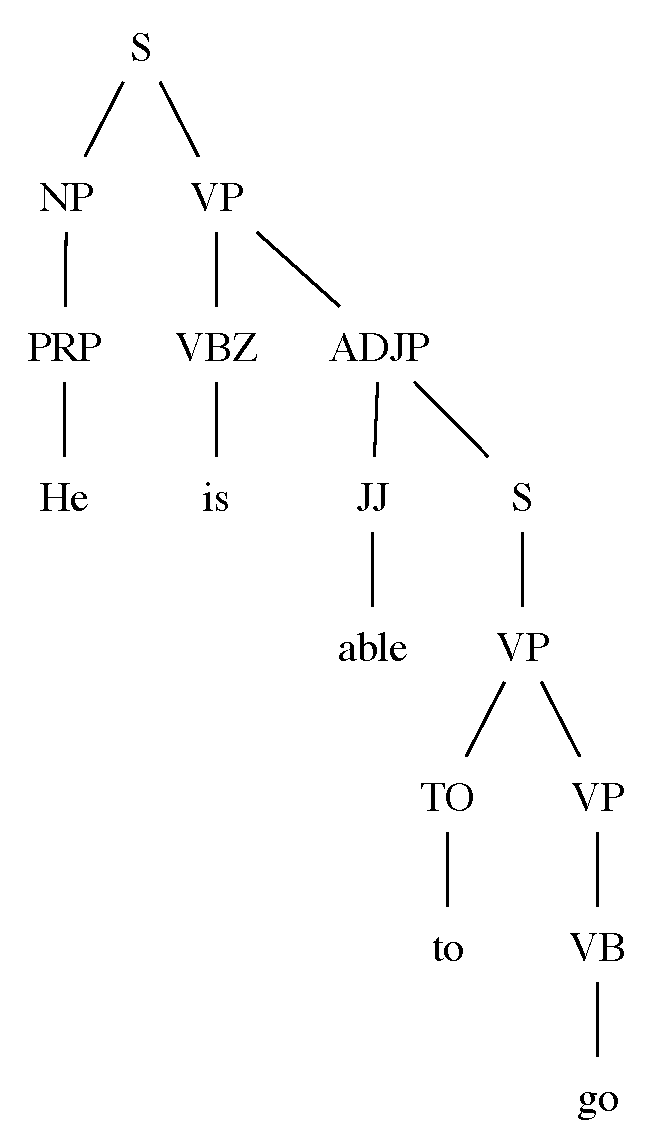
\includegraphics[scale=0.6]{modal-able.pdf}
\caption{Parse Tree Showing Phrasal Modal \textit{be able to.}}
\label{fig:quasimodal-able}
\end{figure}

\begin{figure}[htbp]
\centering
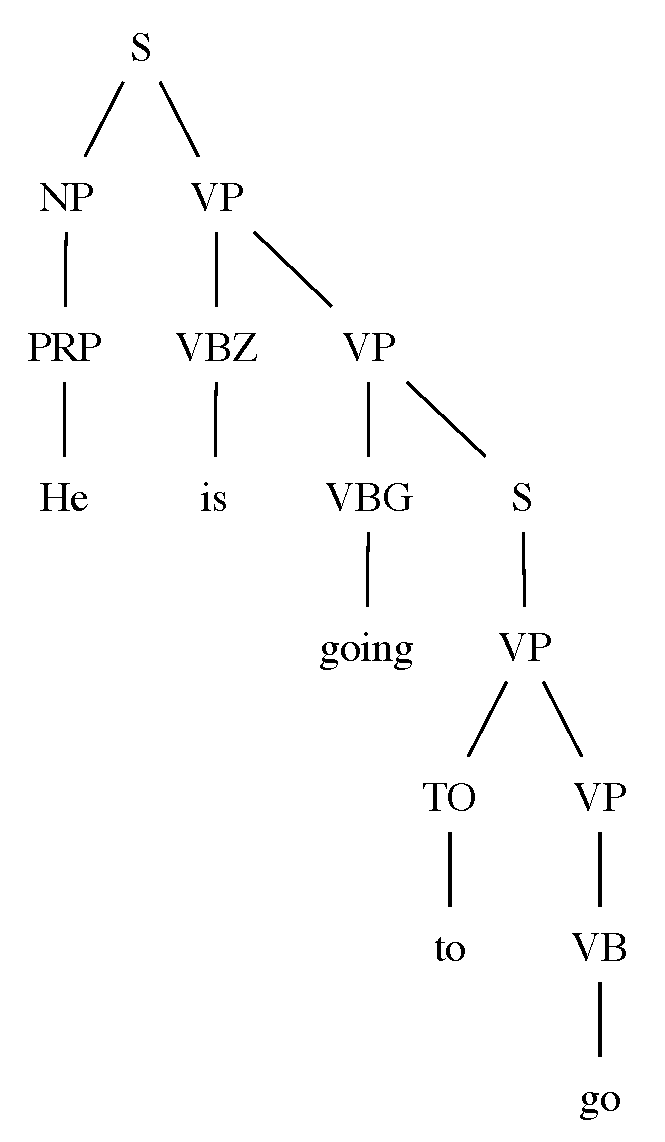
\includegraphics[scale=0.6]{modal-going.pdf}
\caption{Parse Tree Showing Phrasal Modal \textit{be going to.}}
\label{fig:quasimodal-going}
\end{figure}

Phrasal modals are identified by searching parse trees for subtrees that match the basic form of the VP subtrees shown in Figures~\ref{fig:quasimodal-able} and \ref{fig:quasimodal-going}, and of other similar trees, while allowing for variation where appropriate. For instance, to match an instance of \textit{be going to}, a subtree must be found that matches the most dominant VP subtree in Figure~\ref{fig:quasimodal-going}, with the exception that where the leaf [\textit{go}] is found in the model, there may be any terminal node, and where the subtree [VBZ~---~\textit{is}] is found, there may be any subtree representing a conjugation of \textit{be} (e.g., [VBD~---~\textit{was}], [VBP~---~\textit{am}], etc.) The other phrasal modals and constructions using the auxiliary verbs \textit{do}, \textit{have}, and \textit{be} are similarly identifiable using other distinctive subtrees.

Whenever the conjunction \textit{and} is encountered in a VP subtree, multiple distinct but overlapping subtrees are generated from this and treated independently. For instance, the parse of the sentence \textit{he can design and build houses} shown in Figure~\ref{fig:conj-verb} is processed to generate the two separate parses \textit{he can design houses} and \textit{he can build houses} shown in Figure~\ref{fig:conj-verb-ab}. The exception to this is when the conjunction is used to apply multiple modals to a verb (e.g. \textit{I can and will\ldots}).
\begin{figure}[htbp]
\centering
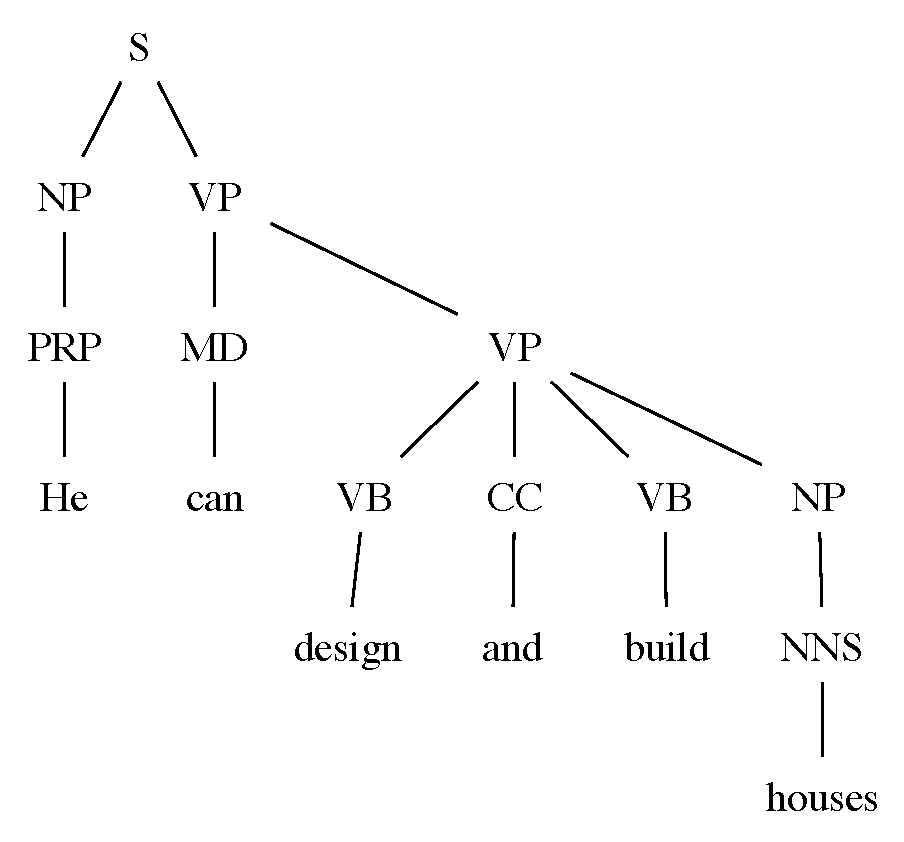
\includegraphics[scale=0.6]{conj-verb.pdf}
\caption{Parse Tree Showing a Verb with Embedded Conjunction}
\label{fig:conj-verb}
\end{figure}

\begin{figure}[htbp]
\centering
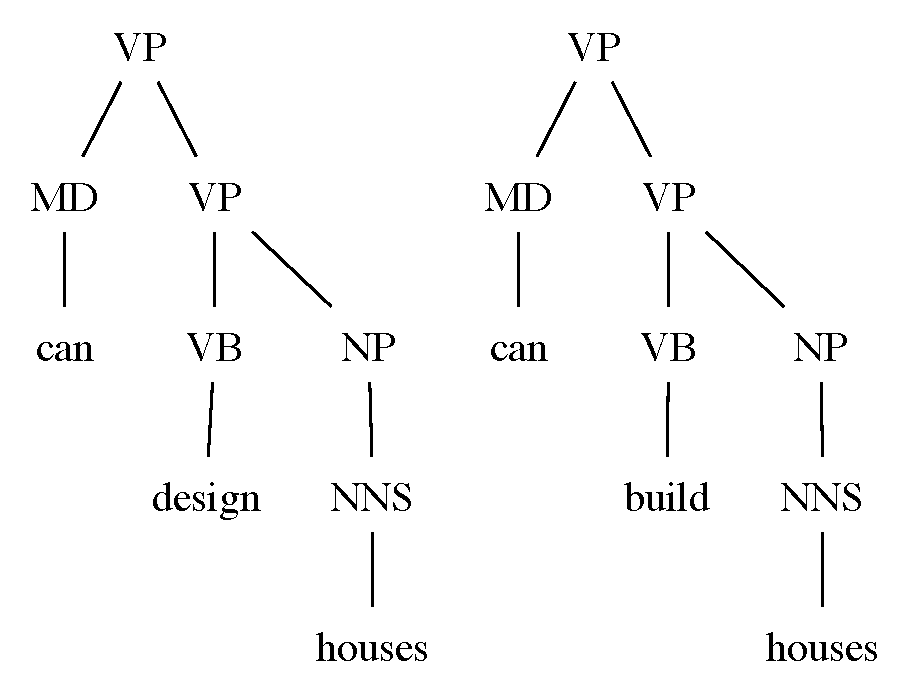
\includegraphics[scale=0.6]{conj-verb-ab.pdf}
\caption{Parse Trees Showing the VP from Figure~\ref{fig:conj-verb} Split into Two VPs}
\label{fig:conj-verb-ab}
\end{figure}

In all, this system uses 169 model subtrees to match the various possible supported verb configurations. It identifies the following binary independent attributes: the past tense, the perfect aspect, the progressive aspect, the passive voice, the presence of the auxiliary \textit{do}, and whether it is negated with \textit{not}. It also identifies any and all modals, the presence and identity of a phrasal modal, and the core verb.

\subsection{Classification}
Being able to identify so many attributes gives a wealth of data with which a classifier may be trained. The challenge, as always, is choosing subsets of this data that maximize information content while still producing decision trees comprehensible to a human. The first such subset examined here consists of eight attributes, each with a value indicating the relative frequency with which such verbal qualities are found in a text. These eight attributes are named ``not,'' ``modal,'' ``progressive,'' ``past,'' ``perfect,'' ``passive,'' ``quasimodal,'' and ``do.'' For the most part these are self-explanatory, with ``not'' being the relative frequency of the negating adverb \textit{not} and so forth (``quasimodal'' indicates a phrasal modal). It is worth pointing out that with the exception of ``modal,'' these verbal attributes can only occur once per verbal construction, but of course all can appear many times in a given text. 

\begin{figure}[htbp]
\centering
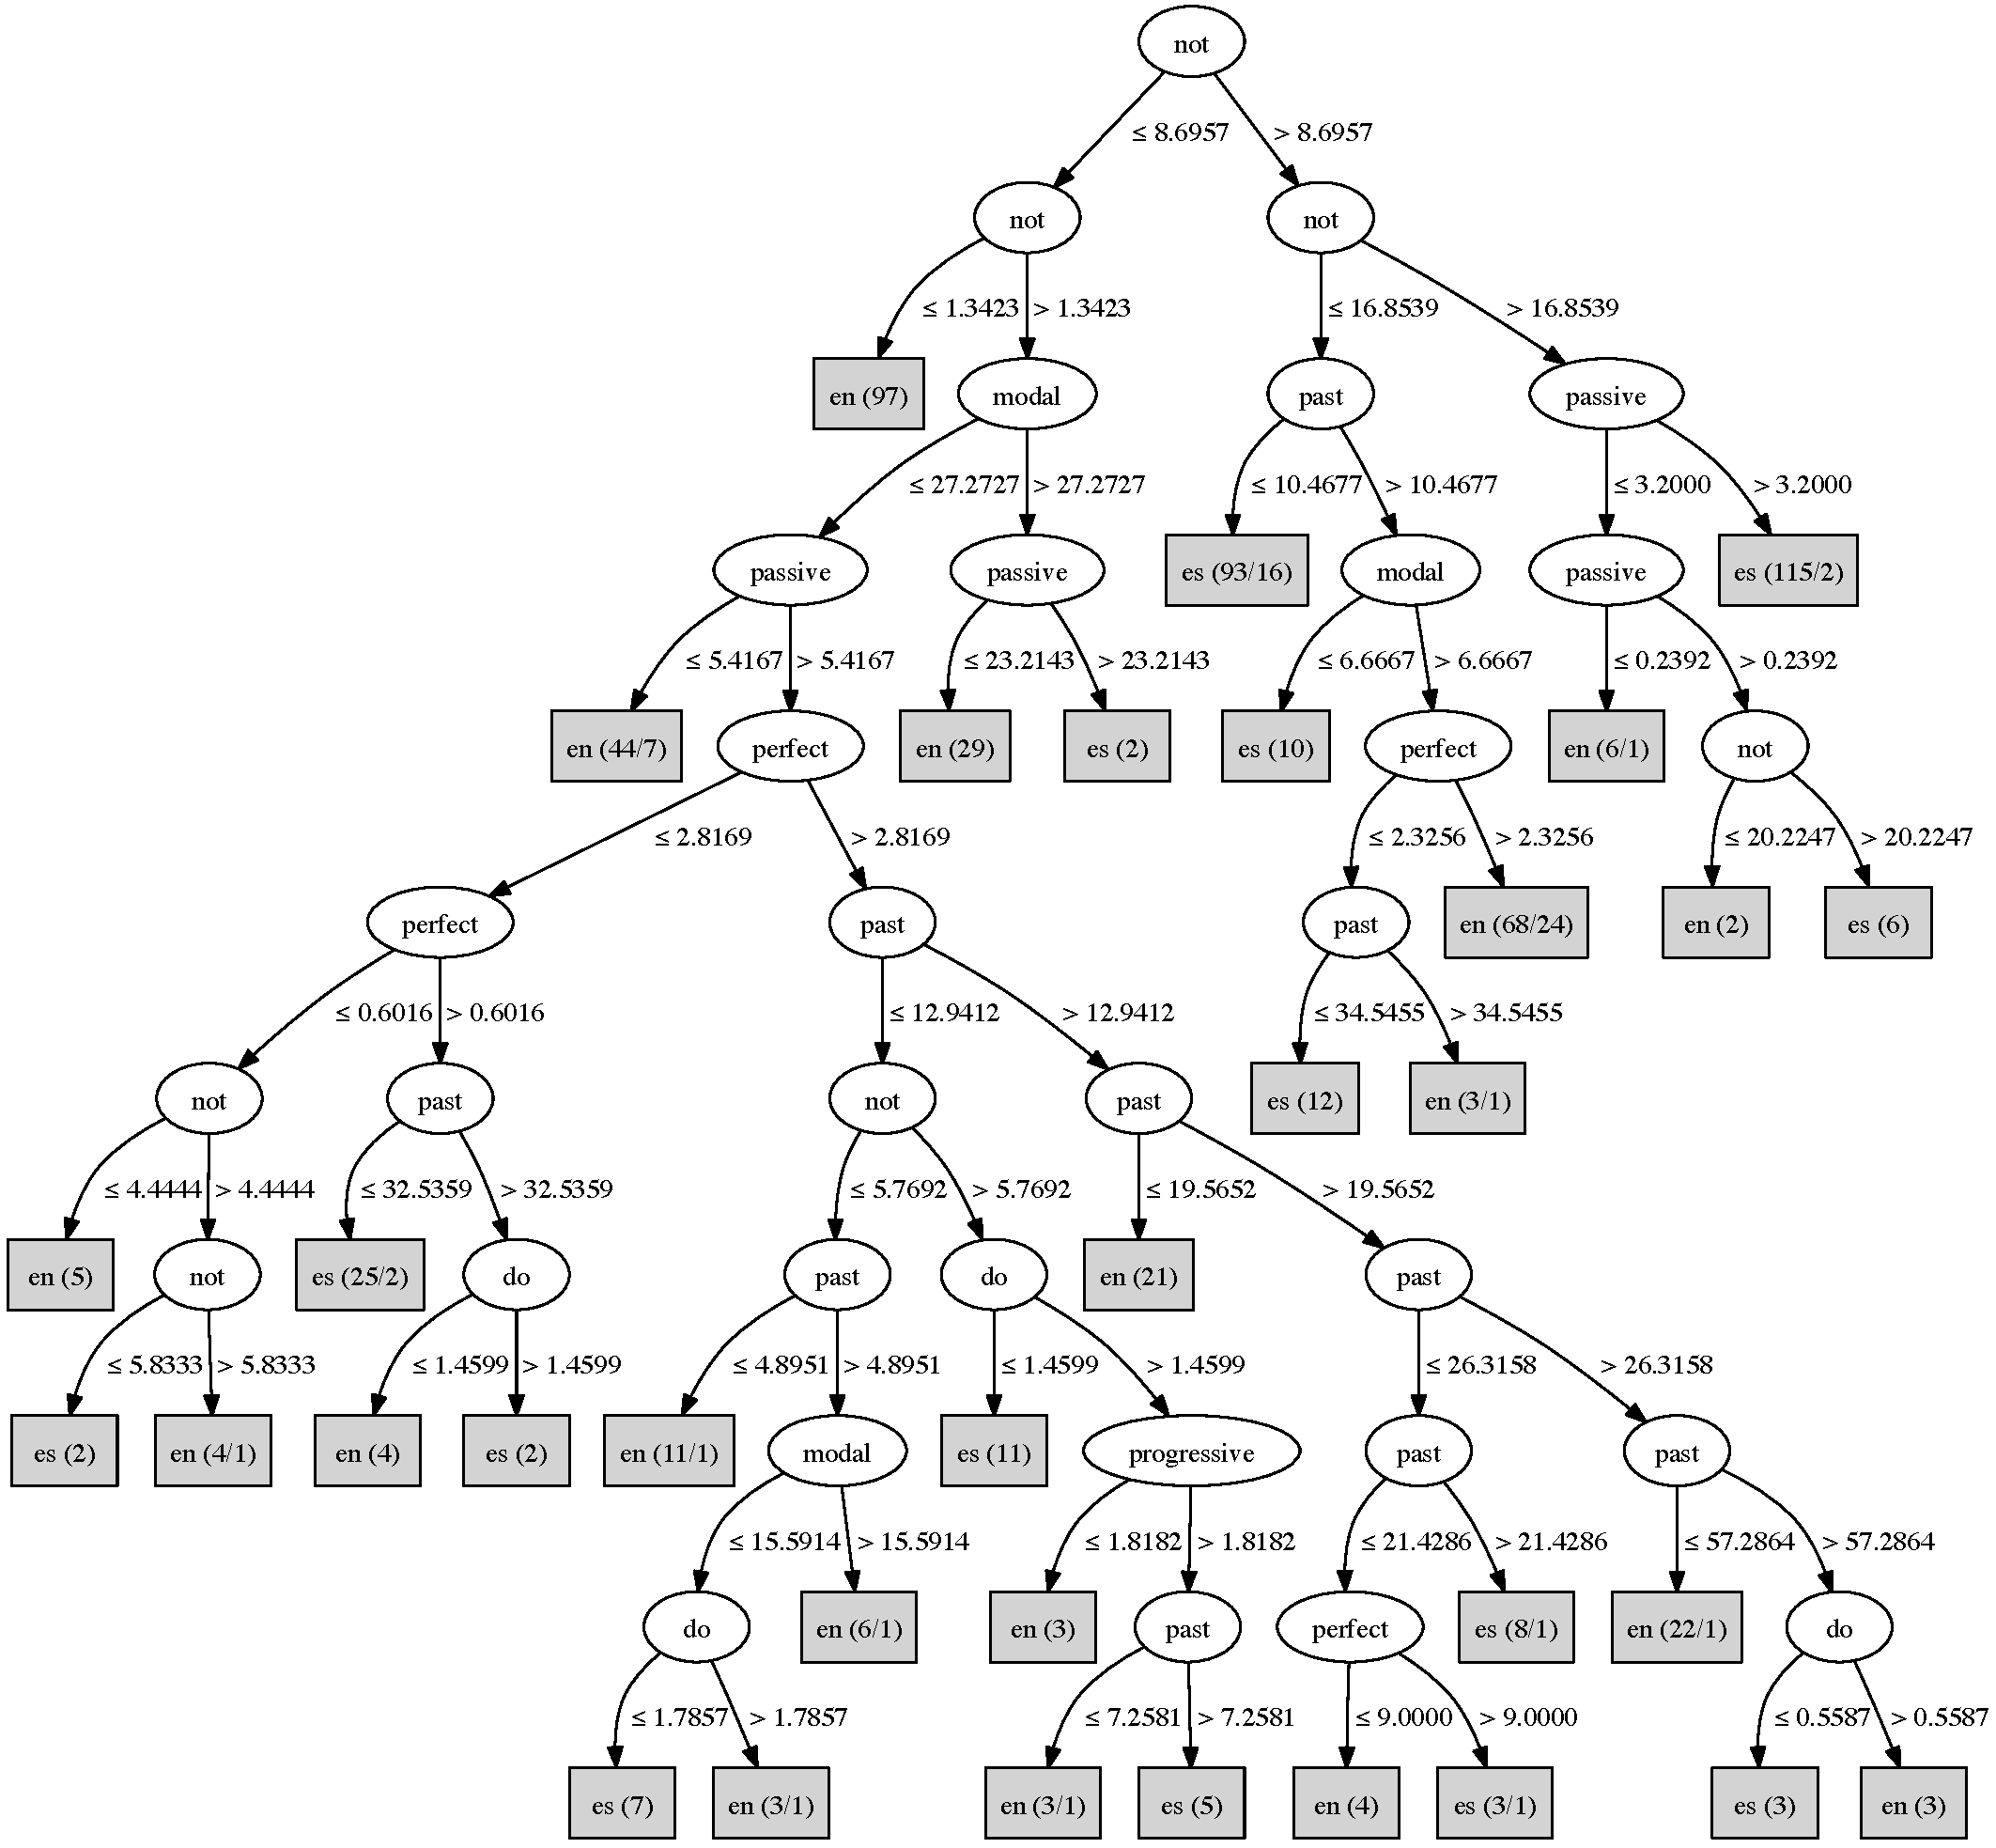
\includegraphics[width=6in]{unpruned-basic-verb-tree.pdf}
\caption{C4.5 Decision Tree Using Various Verbal Attributes With Default Pruning}
\label{fig:normally-pruned-basic-verb-tree}
\end{figure}

\begin{table}[htbp]
\centering
\caption{Accuracy of C4.5 Classifier Using Various Verbal Attributes With Default Pruning}
\begin{tabular}{l c}
\toprule
Nonnative & 71.7\% \\
Native & 81.9\% \\
Overall & 76.8\% \\
Overall C.I. 95\% & 73.5\% --- 80.1\%\\
\bottomrule
\end{tabular}
\label{table:normally-pruned-basic-verb-results}
\end{table}

A C4.5 decision tree generated from this data set is shown in Figure~\ref{fig:normally-pruned-basic-verb-tree} and the accuracy of such classifiers, calculated using 20-fold cross-validation, is shown in Table~\ref{table:normally-pruned-basic-verb-results}. As can be seen, this is quite a large tree for purposes of analysis, with many attributes appearing multiple times. A somewhat simpler tree, with only a modest lost of accuracy, can be had by using more aggressive pruning following the tree construction phase. Figure~\ref{fig:pruned-basic-verb-tree} shows such a tree, and Table~\ref{table:pruned-basic-verb-results} its accuracy. This tree consists of 13 decision nodes considering 6 different attributes, none of which are considered more than three times.
\begin{figure}[htbp]
\centering
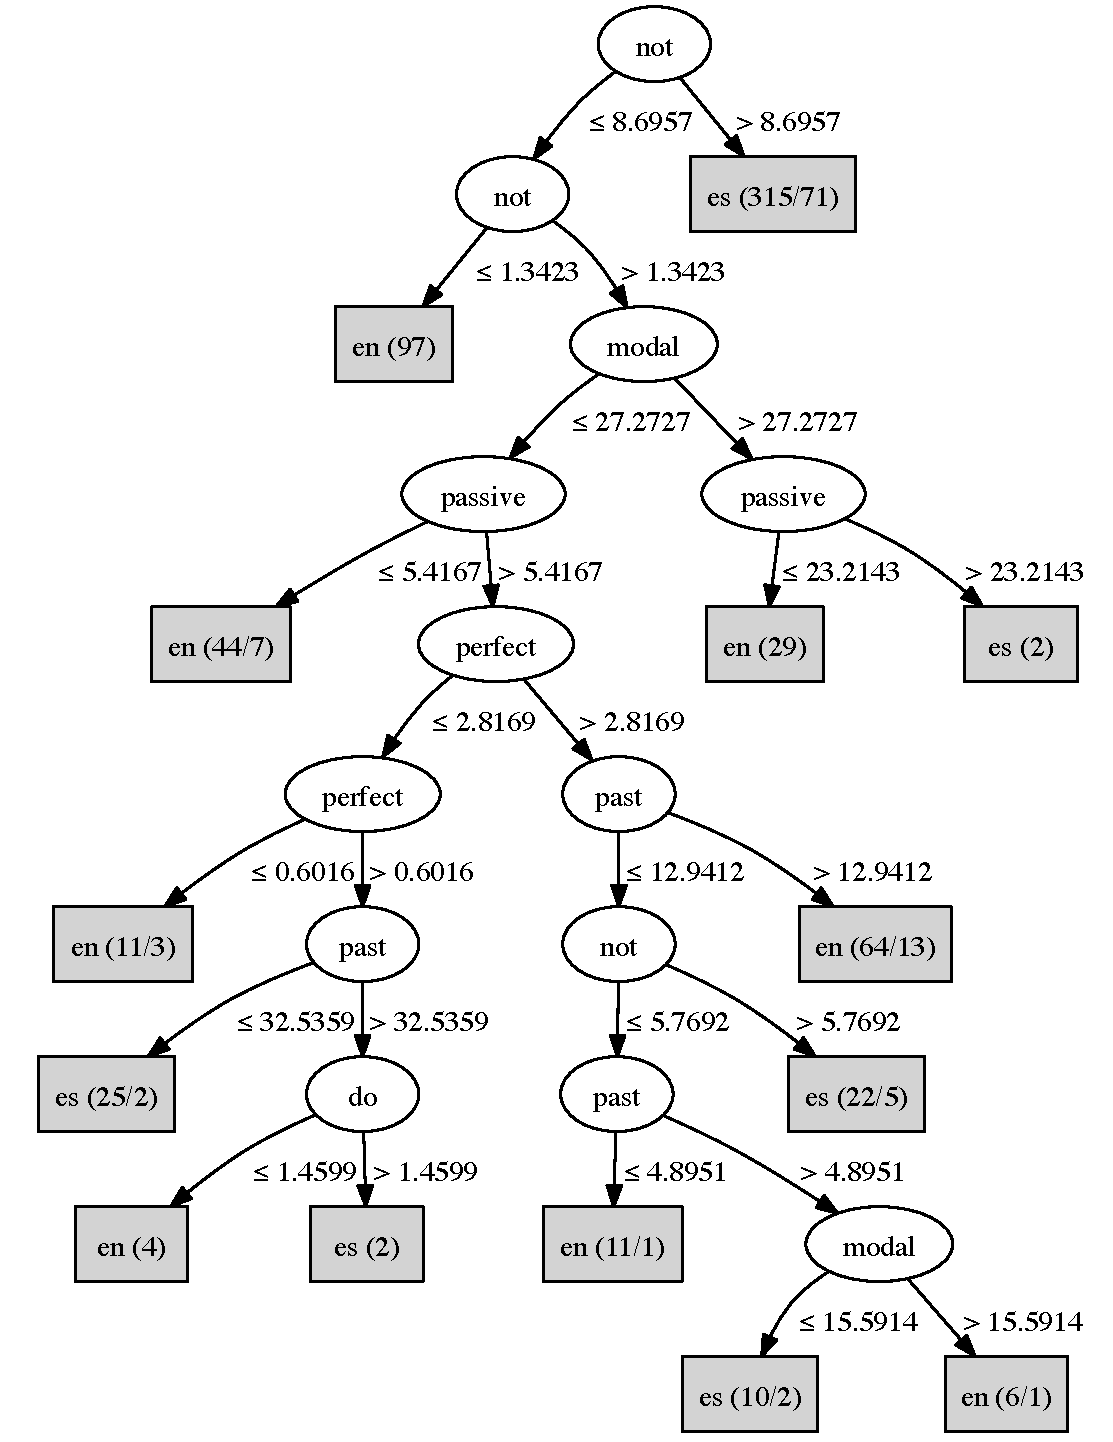
\includegraphics[width=4in]{pruned-basic-verb-tree.pdf}
\caption{Aggressively Pruned C4.5 Decision Tree Using Various Verbal Attributes}
\label{fig:pruned-basic-verb-tree}
\end{figure}
\begin{table}[htbp]
\centering
\caption{Accuracy of Agressively-Pruned C4.5 Classifier Using Various Verbal Attributes}
\begin{tabular}{l c}
\toprule
Nonnative & 71.3\% \\
Native & 79.8\% \\
Overall & 75.5\% \\
Overall C.I. 95\% & 72.2\% --- 78.9\%\\
\bottomrule
\end{tabular}
\label{table:pruned-basic-verb-results}
\end{table}
Of the eight attributes used in training, ``quasimodal'' and ``progressive'' are not found in the aggressively pruned tree, nor does ``quasimodal'' appear in the normally-pruned tree. ``Modal,'' however, does appear in both trees. In the aggressively-pruned tree it appears twice, once very near the root of the tree and the other time as the deepest decision node. The first of these splits the training cases into a predominately nonnative subset, those with frequencies higher than 27.2727\%, and a predominately native subset with lower values. The second decision node, however, uses a lower comparison value and splits the cases the other way, with low values being classified as nonnative. This would seem to indicate that extremes in modal usage are associated with nonnative usage. Before attempting to explain this, it is worth exploring the role of modal verbs in Spanish. According to the analysis of \citet{butt}, Spanish has a small array of modal verbs, in general similar syntactically to English phrasal modals, as shown in the following examples:
\eenumsentence{
\singlespacing
\item \shortex{5}
{\textit{No}&\textit{debiste}&\textit{hacerlo}.}
{\textit{Not}&\textit{you-should-have}&\textit{done-it}.}
{`\textit{You shouldn't have done it.}'}
\item \shortex{5}
{\textit{Hubo}&\textit{de}&\textit{repetir}&\textit{el}&\textit{experimento}.}
{\textit{(S)he-had-to}&&\textit{repeat}&\textit{the}&\textit{experiment}.}
{`\textit{(S)he had to repeat the experiment'}}\\ \citep[Ch. 21.3,21.4]{butt}}
Some of these are usually translated into English using modals or phrasal modals, and some require the use of other constructions \citep[Ch. 21]{butt}. Conversely, many English modals and phrasal modals can be translated into Spanish using that language's modals, while others translate as verbal inflections. In addition, for those Spanish modals which can be translated into English modals or phrasal modals, the correspondence is rarely one-to-one, with there being a great deal of overlap and inexactness in meaning both ways. This should not be surprising, considering the close but imperfect correspondence between many of English's modals and phrasal modals (e.g. \textit{can} and \textit{be able to}) \citep[Ch. 8]{celce-murcia:1999}.

As mentioned above, the Spanish modals have much in common with the English phrasal modals. In general, the pattern of usage of the Spanish modals is \textit{conjugated modal verb} + \textit{one or zero particles} + \textit{infinitive}. As was seen in Table~\ref{table:quasimodal-verbs}, many of the English phrasal modals follow this pattern as well. With a few exceptions, the Spanish modals can take the full range of verbal inflections, as can the majority of English phrasal modals. From this one might assume that L1-Spanish learners of English would take naturally to the English phrasal modal. Indeed, the decision trees shown in Figures~\ref{fig:normally-pruned-basic-verb-tree} and \ref{fig:pruned-basic-verb-tree} would seem to support this, or at least support the proposition that the learners neither overuse nor underuse phrasal modals relative to their native counterparts. A quick experiment in which the C4.5 classifier was run on the same data set, but with the ``modal'' attribute removed, showed that the ``quasimodal'' attribute was still not used in the resultant decision tree. This means that the reason for the algorithm's excluding the ``quasimodal'' attribute cannot be attributed to its containing no information beyond what the ``modal'' attribute contains.

Returning to the ``modal'' attribute, it was mentioned above that the decision tree uses overuse and underuse of the English simple modals as an indication that the text being analyzed was written by a learner. Unfortunately, there is surprisingly little literature on the acquisition of English modals by Spanish speakers, but it is not difficult to imagine situations that would lead learners to either overuse or underuse modals. A learner might avoid the English modal, it being syntactically unusual from a Spanish grammar perspective, or, having discovered the relative simplicity of the English modal, which requires no verbal inflection, may use it to excess. The data also suggests that some learners avoid all types of modals.

In Figure~\ref{fig:pruned-basic-verb-tree}, it could be seen that the attribute with the highest information content is ``not.'' This is used three times, with higher frequencies tending to lead to classification as nonnative and lower frequencies to native. It is tempting to attribute this to Spanish's double negative construction \citep[ch. 23.3]{butt}, but it seems doubtful that advanced English learners would not have grasped this basic difference between English and Spanish grammar. More likely is that native speakers, with their presumably larger vocabularies, have a greater number of lexical negatives (e.g. \textit{he is unkind} versus \textit{he is not kind}) at their disposal.

Considering next the ``passive'' attribute, it can be seen that this attribute, too, is used in a consistent manner in the decision tree, with lower and higher frequencies leading to classification as native and nonnative, respectively. Spanish expresses passives in primarily two ways: using the copular verb \textit{ser} plus a past participle in a construction similar to the English passive, or, more commonly, using the reflexive pronoun \textit{se}:
\eenumsentence{
\singlespacing
\item \shortex{5}
{\textit{Las}&\textit{muestras}&\textit{les}&\textit{serán}&\textit{devueltas}.}
{\textit{The}&\textit{samples}&\textit{to-you} (pl.)&\textit{will-be}&\textit{returned}.}{}
\item \shortex{5}
{\textit{Se}&\textit{les}&\textit{devolverán}&\textit{las}&\textit{muestras}.}
{&\textit{to-you} (pl.)&\textit{will-return}&\textit{the}&\textit{samples}.}
{`\textit{The samples will be returned to you.}'}\\ \citep[p. 402,8]{butt}}
Based on these constructions, it is not surprising that L1-English learners of Spanish tend to overuse the \textit{ser}-passive \citep[ch. 28.2.3]{butt}. That L1-Spanish learners of English do the same with the \textit{be}-passive is more surprising. Indeed, this author was unable to find any literature that investigates, or even acknowledges, this phenomenon. One possibility has to do with the connection between the English passive and the presentation of information at the discourse level. The English passive is frequently used to reverse the order of what, in an active sentence, would be the subject and object. Such a reversal is often necessary to preserve the tendency in language to present old information before new information. However, the passive is only one of a number of constructions, the least marked such construction, perhaps, that allow the fronting of a particular element in a sentence \citep{ward:2008}. Other such constructions (e.g. preposing, inversion), being more complicated and alien, may be avoided by the learner, leading to an overuse of the passive.

The remaining three attributes used in the decision tree are rather resistant to analysis. The perfect aspect constructions in English and Spanish, for instance, are remarkably similar, with English using a form of the verb \textit{to have} plus the past participle and Spanish using a form the verb \textit{haber} (cf. Latin \textit{habere}, \textit{to have}), plus a past participle. That the frequency of usage of the perfect should be a useful metric in classification is surprising. Similarly, English and Spanish both have inflected past tenses which, combined with the complex role the ``past'' attribute plays in the decision tree, makes deciphering that attribute difficult. Finally, while Spanish has nothing quite like English's \textit{do} auxiliary, the extremely limited role which the ``do'' attribute plays in the classification process (it is only involved in classifying six out of 642 training cases) suggests that it is of little utility.

The next set of attributes deals with the relative frequencies of the various possible modals and phrasal modals. Table~\ref{table:quasimodal-verbs} shows the phrasal modals parsed in this system, of which there are 13; and Table~\ref{table:modal-verbs} shows the modals, of which there are 9. This yields a total of 22 attributes. Training a C4.5 classifier on this data set produces a decision tree which is rather opaque in terms of interpretation, but the accuracy of such a classifier can be see in Table~\ref{table:modal-attributes-results}. 
\begin{table}[htbp]
\centering
\caption{Accuracy of C4.5 Classifier Using Modal Attributes}
\begin{tabular}{l c}
\toprule
Nonnative & 76.1\% \\
Native & 73.8\% \\
Overall & 74.9\% \\
Overall C.I. 95\% & 71.6\% --- 78.3\%\\
\bottomrule
\end{tabular}
\label{table:modal-attributes-results}
\end{table}
A derivative data set, which sacrifices accuracy for interpretability, produces the C4.5 tree shown in Figure~\ref{fig:modal-phrasal-tree}. The attributes used in this tree indicate whether there is a tendency in a text to use a modal over a phrasal modal with a similar meaning. Only four attributes were used, derived from a total of eleven modals and phrasal modals. Table~\ref{table:modal-phrasal-correspondence}\footnote{For unspecified reasons, \citet{butt} does not include \textit{ir a} with the modals. This is likely for the same reason that many English grammars do not consider \textit{will} a modal, presumably because it modifies tense and not mood.} shows the modals used and the corresponding phrasal modals. The values for these attributes were calculated by subtracting from the number of occurrences of a particular modal the number of occurrences of the corresponding phrasal modals, and dividing the difference by the sum of these two quantities. This yields a real number ranging from $-1$ to $1$, with the most negative number indicating all phrasal modals and no modals, zero indicating an even number of each, and $1$ indicating all modals and no phrasal modals. For the purposes of display in Figure~\ref{fig:modal-phrasal-tree}, these numbers are scaled by a factor of 100. The labels given to the attributes are the names of the modal, these being unique for each correspondence.
\begin{table}[htbp]
\centering
\caption{Correspondence Between Modals and Phrasal Modals}
\begin{tabular}{l l l}
\toprule
Modal & Phrasal Modal & Spanish Modal\\
\midrule
\textit{can} &
\begin{tabular}{>{\itshape}l}
be able to
\end{tabular}
&
\begin{tabular}{>{\itshape}l}
poder
\end{tabular}\\
\midrule
\textit{must} &
\begin{tabular}{>{\itshape}l}
have to\\have got to\\need to\\
\end{tabular} &
\begin{tabular}{>{\itshape}l}
tener que\\deber\\haber que\\
\end{tabular}\\
\midrule
\textit{should}&
\begin{tabular}{>{\itshape}l}
ought to\\be supposed to\\be obliged to\\
\end{tabular} &
\begin{tabular}{>{\itshape}l}
deber\\haber de\\
\end{tabular}\\
\midrule
\textit{will}&
\begin{tabular}{>{\itshape}l}
be going to\\
\end{tabular} &
\begin{tabular}{>{\itshape}l}
ir a\\
\end{tabular}\\
\bottomrule
\end{tabular}
\label{table:modal-phrasal-correspondence}
\end{table}
\begin{figure}[htbp]
\centering
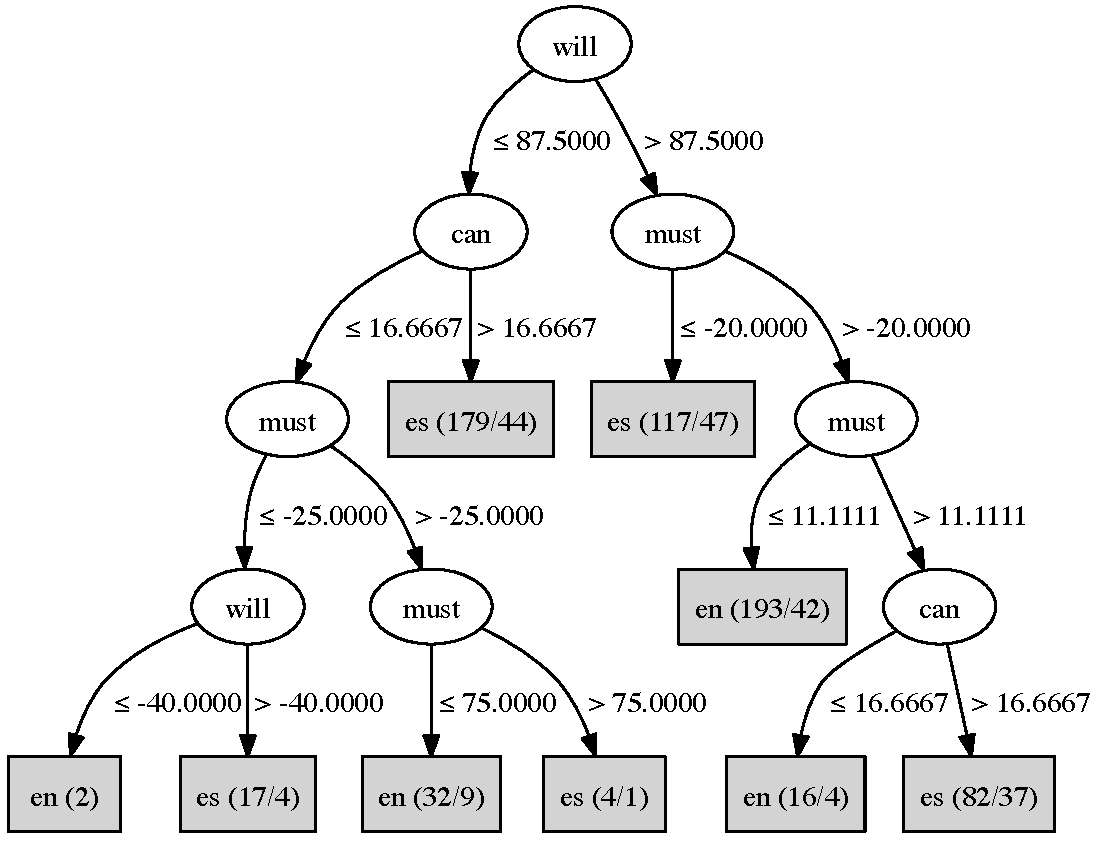
\includegraphics[width=4in]{modal-phrasal-tree.pdf}
\caption{C4.5 Decision Tree Using Modal vs Phrasal Attributes}
\label{fig:modal-phrasal-tree}
\end{figure}
\begin{table}[htbp]
\centering
\caption{Accuracy of C4.5 Classifier Using Modal vs Phrasal Attributes}
\begin{tabular}{l c}
\toprule
Nonnative & 70.7\% \\
Native & 61.4\% \\
Overall & 66.0\% \\
Overall C.I. 95\% & 62.3\% --- 69.7\%\\
\bottomrule
\end{tabular}
\label{table:modal-phrasal-results}
\end{table}

The resultant tree uses three of the four attributes, with the ``should'' attribute not being included. The tree indicates that there is a strong tendency for the learners to use core modals more often relative to phrasal modals than the native writers. This is despite the similarity between English phrasal modals and Spanish modals. Table~\ref{table:modal-phrasal-correspondence} also shows common Spanish modal equivalents to the English modals and phrasal modals. As can be seen from this table, each of these English modals can be expressed using a common Spanish modal, including \textit{will}/\textit{be going to}, which has a Spanish modal equivalent that is used alongside Spanish's inflected future \citep[ch. 14.6.4]{butt}. The best explanation for this is that learners prefer the core modals due to their syntactic simplicity.

The third set of attributes considers various common English verbs which are shown in Table~\ref{table:high-freq-verbs}.
\begin{table}[htbp]
\centering
\caption{High Frequency Verbs}
\begin{tabular}{>{\itshape}l >{\itshape}l >{\itshape}l >{\itshape}l >{\itshape}l}
\toprule
make & use & take & see & say\\
go & become & believe & give & feel\\
come & find & think & know & look\\
seem & want & get & live & work\\
\bottomrule
\end{tabular}
\label{table:high-freq-verbs}
\end{table}
These verbs are identified as common verbs that tend to be overused by English learners in a study by \citet{ringbom:1998}. This study uses an earlier version of the ICLE, examining the French, Spanish, Finnish, Swedish, Dutch, and German subcorpora for usages of these verbs, and comparing the frequency of usage to that found in a native subcorpus of the ICLE\footnote{The version of ICLE used in the present study contains no native subcorpus.}. \citeauthor{ringbom:1998} gives the breakdown per word, and finds that not all of the verbs show overuse in the Spanish subcorpus, with only \textit{use, believe, feel}, and \textit{come} showing overuse. \citeauthor{ringbom:1998} does not attempt to establish statistical significance, however. These verbs were used to construct a data set consisting of one attribute per verb with the value of each being equal to the relative frequency of that verb when used as a main verb in a finite clause. The accuracy of a C4.5 classifier trained on this data set is shown in Table~\ref{table:high-freq-results}.
\begin{table}[htbp]
\centering
\caption{Accuracy of C4.5 Classifier Using High Frequency Verb Attributes}
\begin{tabular}{l c}
\toprule
Nonnative & 65.4\% \\
Native & 78.8\% \\
Overall & 72.1\% \\
Overall C.I. 95\% & 68.6\% --- 75.6\%\\
\bottomrule
\end{tabular}
\label{table:high-freq-results}
\end{table}

Finally, to gauge the efficacy of verbal attributes in general, classifiers were trained on a combined data set consisting of all four sets of verbal attributes discussed here. Both a C4.5 classifier and a random forest classifier was tried. The accuracy of these classifiers is shown in Table~\ref{table:c45-combined-results} and Table~\ref{table:combined-results}.
\begin{table}[htbp]
\centering
\caption{Accuracy of C4.5 Classifier Using All Verbal Attributes}
\begin{tabular}{l c}
\toprule
Nonnative & 80.4\% \\
Native & 77.3\% \\
Overall & 78.8\% \\
Overall C.I. 95\% & 75.7\% --- 82.0\%\\
\bottomrule
\end{tabular}
\label{table:c45-combined-results}
\end{table}
\begin{table}[htbp]
\centering
\caption{Accuracy of Random Forest Classifier Using All Verbal Attributes}
\begin{tabular}{l c}
\toprule
Nonnative & 90.3\% \\
Native & 85.4\% \\
Overall & 87.9\% \\
Overall C.I. 95\% & 85.3\% --- 90.4\%\\
\bottomrule
\end{tabular}
\label{table:combined-results}
\end{table}
Combining the various attributes sets results in an approximately 4\% improvement in accuracy over using just the modal attributes, which have the highest accuracy of any of the attribute sets. However, one should note that the confidence intervals for the two classifiers do overlap somewhat, which would lead the cautious statistician to conclude that there is insufficient evidence to assert that one is better than the other at the 95\% confidence level. At slightly lower confidence levels, however, there would be no overlap. Using a random forest classifier improves that accuracy by nearly 10\%.
\biblio
\end{document}